\chapter{Maximum Likelihood Estimation}
\section{Maximum Likelihood in Machine Learning}

In our statistical perspective on error, we decompose the error into three components: the bias of our predictions, the variance of our learning algorithm, and the inherent noise in our observations. The final term arises when decomposing our model's bias but was not fully aligned with our machine learning perspective, as we had not yet considered our observations \( y \) to be noisy. Additionally, in our statistical analysis of model errors, we contemplated the effect of resampling the entire dataset. Consequently, we now view the dataset
\[
    \mathcal{D} = \{(\boldsymbol{x}^{(i)}, \boldsymbol{y}^{(i)})\}_{i=1}^{k}
\]
as being sampled from random variables:
\[
    \mathcal{D} = \{(x^{(i)}, y^{(i)}) \sim P(\mathbf{x}_i, \mathbf{y}_i)\}_{i=1}^{k}.
\]
While treating the dataset as random may initially seem more complex, we begin our analysis by assuming a linear model and a known distribution of label noise, specifically that it is normally distributed as \( \mathcal{N}(0, \sigma^2) \). This assumption defines our probabilistic model. Under this assumption, the model's output at a point is given by
\[
    \hat{\mathbf{y}} = \boldsymbol{X}\theta + \epsilon, \quad \epsilon \sim \mathcal{N}(0, \sigma^2).
\]
Here, the output \( \hat{\mathbf{y}} \) is a random variable, which introduces the need to employ probabilistic tools in the learning process. The distribution of \( \hat{\mathbf{y}} \) is therefore
\[
    \hat{\mathbf{y}} \sim \mathcal{N}(\boldsymbol{x}^{(i)\top}\theta, \sigma^2).
\]
This distribution models our assumptions about the noise in our observations. Given the dataset \( \mathcal{D} \), we seek parameter values \( \theta \) that maximise the likelihood of observing the data. For two different parameters \( \theta \) and \( \theta' \), we prefer \( \theta \) if
\[
    p(\hat{\mathbf{y}} = \boldsymbol{y}^{(i)} \mid \theta, \boldsymbol{x}^{(i)}) > p(\hat{\mathbf{y}} = \boldsymbol{y}^{(i)} \mid \theta', \boldsymbol{x}^{(i)}).
\]
Extending this to all possible parameters \( \theta \in \Theta \), the parameter that maximises the likelihood is
\[
    \theta^{\star} = \underset{\theta \in \Theta}{\mathrm{argmax}} \, p(\mathcal{D} \mid \theta).
\]
The term \( p(\mathcal{D} \mid \theta) \) is known as the \textbf{likelihood}, and \( \theta^{\star} \) is referred to as the \textbf{maximum likelihood estimate} (MLE). To express the likelihood for the entire dataset, assuming that the data points are independently and identically distributed (i.i.d.), we have
\[
    p(\mathcal{D} \mid \theta) = \prod_{i=1}^{k} p(\hat{\mathbf{y}} = \boldsymbol{y}^{(i)} \mid \theta, \boldsymbol{x}^{(i)}).
\]
For our linear model with Gaussian noise, this becomes
\[
    p(\mathcal{D} \mid \theta) = \prod_{i=1}^{k} \mathcal{N}(\boldsymbol{y}^{(i)} \mid \theta^\top \boldsymbol{x}^{(i)}, \sigma^2).
\]
Expanding the normal density, the likelihood is
\[
    p(\mathcal{D} \mid \theta) = \prod_{i=1}^{k} \frac{1}{\sqrt{2\pi\sigma^2}} \exp\left( -\frac{1}{2\sigma^2} (\mathbf{y}^{(i)} - \boldsymbol{x}^{(i)\top}\theta)^2 \right).
\]
This expression can be simplified by noting that the constant term \( \frac{1}{\sqrt{2\pi\sigma^2}} \) can be factored out:
\[
    p(\mathcal{D} \mid \theta) = \frac{1}{(2\pi\sigma^2)^{k/2}} \exp\left( -\frac{1}{2\sigma^2} \sum_{i=1}^{k} (\mathbf{y}^{(i)} - \boldsymbol{x}^{(i)\top}\theta)^2 \right).
\]
To find the MLE, we seek to maximise the log-likelihood:
\[
    \log p(\mathcal{D} \mid \theta) = -\frac{k}{2} \log(2\pi\sigma^2) - \frac{1}{2\sigma^2} \sum_{i=1}^{k} (\boldsymbol{y}^{(i)} - \boldsymbol{x}^{(i)\top}\theta)^2.
\]
Maximising the log-likelihood is equivalent to minimising the negative log-likelihood:
\[
    -\log p(\mathcal{D} \mid \theta) = \frac{k}{2} \log(2\pi\sigma^2) + \frac{1}{2\sigma^2} \sum_{i=1}^{k} (\boldsymbol{y}^{(i)} - \boldsymbol{x}^{(i)\top}\theta)^2.
\]
Ignoring constant terms that do not depend on \( \theta \), this minimisation problem reduces to the ordinary least squares (OLS) objective:
\[
    \sum_{i=1}^{k} (\boldsymbol{y}^{(i)} - \boldsymbol{x}^{(i)\top}\theta)^2.
\]
Thus, the MLE for linear regression with Gaussian noise is equivalent to the OLS estimator.


\intuitb{MLE and OLS}{
    The equivalence of MLE and OLS is notable for several reasons. Firstly, unlike OLS, we did not select a loss function; instead, we chose a probabilistic model, and the loss function emerged from the negative log likelihood. Different distributions lead to different loss functions. Additionally, since MLE is equivalent to OLS, it shares the same drawbacks, such as overfitting.
}

\section{Exponential Families}

\marginnote{
    \begin{enumerate}
        \item \textbf{\( \theta \cdot s(x) \)} (or \( \theta^\top s(x) \)):  
        This is called the \textbf{natural parameter weighted sufficient statistic} or simply the \textbf{canonical parameter weighted sufficient statistic}. It is the scalar product of the natural parameter vector \( \theta \) and the sufficient statistic \( s(x) \), capturing the interaction between the data and the parameter in the model.

        \item \textbf{\( h(x) \exp(\theta \cdot s(x)) \)}:  
        This is referred to as the \textbf{unnormalised density} or \textbf{unnormalised probability measure}. It provides the numerator of the exponential family form, where the function \( h(x) \) adjusts for the support of \( x \), and \( \exp(\theta \cdot s(x)) \) adds the exponential weighting based on the parameter-data relationship.  
    \end{enumerate}

    Together with \( z(\theta) \), this forms the complete probability distribution:
    \[
    p(x; \theta) = \frac{h(x) \exp(\theta \cdot s(x))}{z(\theta)}
    \]
}

\defb{Exponential Family}{
    A family of probability distributions where the density can be expressed in the canonical form, where \( \theta \) is the natural parameter:
    \[
        p(\boldsymbol{x}; \theta) = h(\boldsymbol{x}) \exp\left( \sum_{i=1}^m \eta_i(\theta) s_i(\boldsymbol{x}) \right) / z(\theta)
    \]

    We focus on the canonical form, where \( \eta_i(\theta) = \theta_i \), simplifying the general form to a dot product.

    \[
        p(\boldsymbol{x}; \theta) = \frac{h(\boldsymbol{x}) \exp(\theta^\top s(\boldsymbol{x}))}{z(\theta)}
    \]
    Here:
    \begin{itemize}
        \item \( h(\boldsymbol{x}) \): The support function, it determines the support of the distribution to ensure probabilities are non-zero only where appropriate.
        \item \( s(\boldsymbol{x}) \): The sufficient statistic of the data. It is a function of the observed data that encapsulates all information needed to estimate parameter $\theta$. It captures the essential features of the data necessary for the distribution.
        \item \( z(\theta) \): The normalising constant, guaranteeing that the total probability sums to one.
    \end{itemize}



}

The canonical form differs from the general form by setting the natural parameters directly as coefficients in the exponent, facilitating easier mathematical manipulation and interpretation.

\defb{Exponential Distribution}{
    For \( X \sim \text{Exponential}(\lambda) \), the density in the canonical form is:
    \[
        p(x; \theta) = \lambda\exp(-\lambda x)= h(x) \exp(\theta s(x) - z(\theta))
    \]
    where
    \[
        \begin{aligned}
            h(x)      & = \mathbf{I}(x \geq 0), \\
            s(x)      & = x,                    \\
            \theta    & = -\lambda,             \\
            z(\theta) & = -\log(-\theta).
        \end{aligned}
    \]
    $\mb{I}$ is the indicator function that returns 1 if the condition is true and 0 otherwise. \bigskip

    \textbf{Use Cases}: Models the time between independent events in a Poisson process. Examples include predicting the time until an event like system failure, customer churn, or predicting when a customer will cancel their subscription.
}

\defb{Normal Distribution}{
    For \( X \sim \mathcal{N}(\mu, \sigma^2) \), the density in the canonical form is:
    \[
        p(x; \theta) = h(x) \exp(\theta s(x) - z(\theta))
    \]
    where
    \[
        \begin{aligned}
            h(x)      & = \frac{1}{\sqrt{2\pi\sigma^2}}, \\
            s(x)      & = x,                             \\
            \theta    & = \frac{\mu}{\sigma^2},          \\
            z(\theta) & = \frac{\mu^2}{2\sigma^2}.
        \end{aligned}
    \]
    \[
        p(x; \theta) = \frac{1}{\sqrt{2\pi\sigma^2}} \exp \left( -\frac{(x - \mu)^2}{2\sigma^2} \right)
    \]

    \textbf{Use Case}: Represents continuous data with symmetric distribution around the mean, such as heights or measurement errors.
}

\defb{Bernoulli Distribution}{
    For \( X \sim \text{Bernoulli}(p) \), the probability mass function in the canonical form is:
    \[
        p(x; \theta) = h(x) \exp(\theta s(x) - z(\theta))
    \]
    where
    \[
        \begin{aligned}
            h(x)      & = 1,                                \\
            s(x)      & = x,                                \\
            \theta    & = \log\left(\frac{p}{1 - p}\right), \\
            z(\theta) & = \log(1 + e^{\theta}).
        \end{aligned}
    \]
    \[
        p(x; \theta) = p^x (1 - p)^{1-x}
    \]

    \textbf{Use Case}: Models binary outcomes, such as coin toss results or pass/fail scenarios.
}

\section{Generalized Linear Models and the MLE}

With the perspective of probability densities as functions and assuming that all random variables are distributed according to an exponential family, we aim to generalise the probabilistic form of linear models.

\bigskip
Specifically, we maintain the linear combination of features and parameters \( X\theta \), but instead of having \( X\theta \) directly output the mean of a distribution, we introduce a link function to map \( X\theta \) to the appropriate parameter space.

\defb{Link Function}{
    A function that maps the linear combination \( X\theta \) to a parameter of the response distribution, ensuring that the parameter lies within a valid range. For instance, in logistic regression, the link function (usually a sigmoid function for binary classification) maps \( X\theta \) to the interval \([0,1]\).
}

Consider using \( X\theta \) to model the mean of a Bernoulli random variable:
\begin{marginfigure}
    \centering
    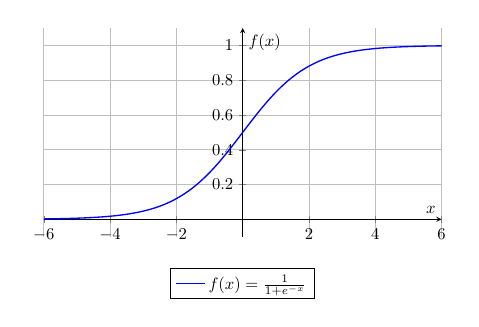
\begin{tikzpicture}[scale=0.6]
        \begin{axis}[
                axis lines=middle,
                grid=both,
                xlabel={$x$},
                ylabel={$f(x)$},
                xmin=-6, xmax=6,
                ymin=-0.1, ymax=1.1,
                domain=-6:6,
                samples=200,
                xtick={-6,-4,-2,0,2,4,6},
                ytick={0,0.2,0.4,0.6,0.8,1},
                width=10cm,
                height=6cm,
                legend style={at={(0.5,-0.15)},anchor=north,legend columns=-1},
                legend cell align={left}
            ]
            \addplot[
                thick,
                smooth,
                blue
            ] {1/(1 + exp(-x))};
            \addlegendentry{$f(x) = \frac{1}{1 + e^{-x}}$}
        \end{axis}
    \end{tikzpicture}
    \caption{The sigmoid function, defined as \( f(x) = \frac{1}{1 + e^{-x}} \)}
    \label{fig:sigmoid}
\end{marginfigure}




\[
    \hat{y}^{(i)} = \boldsymbol{x}^{(i)\top}\theta, \quad p(y^{(i)} = \hat{y}) = \hat{y}^{y^{(i)}} (1 - \hat{y})^{1 - y^{(i)}}.
\]
However, this poses a problem as \( \hat{y}^{(i)} \) can take any real value, making the probability model invalid. To address this, we apply a link function that constrains \( \hat{y}^{(i)} \) to \([0,1]\). The logistic (sigmoid) function is a common choice:
\[
    \sigma(a) = \frac{1}{1 + \exp(-a)}, \quad \text{where } a = \boldsymbol{x}^{(i)\top}\theta.
\]

\defb{Logistic Function}{
    \raggedright
    The logistic function is defined as \( \sigma(a) = \frac{1}{1 + \exp(-a)} \). It is visualised in Figure \ref{fig:sigmoid}. The function's boundedness, symmetry, and smooth gradients make it suitable for optimisation. Alternatives like the probit function may also be used.
}



The function \( \sigma(a) \) serves as the \textbf{link function}, mapping the linear output \( \boldsymbol{x}^{(i)\top}\theta \) to a probability in \([0,1]\). This enables us to define the probability of \( y^{(i)} = 1 \) as:
\[
    p(y^{(i)} = 1 \mid \boldsymbol{x}^{(i)}, \theta) = \sigma(\boldsymbol{x}^{(i)\top}\theta) = \frac{1}{1 + \exp(-\boldsymbol{x}^{(i)\top}\theta)}.
\]

For a given label \( y^{(i)} \), the probability is:
\[
    p(y^{(i)} \mid \boldsymbol{x}^{(i)}, \theta) = \sigma(\boldsymbol{x}^{(i)\top}\theta)^{y^{(i)}} \cdot (1 - \sigma(\boldsymbol{x}^{(i)\top}\theta))^{1 - y^{(i)}}.
\]

Thus, the likelihood function for the entire dataset \( \mathcal{D} = \{(\boldsymbol{x}^{(i)}, y^{(i)})\}_{i=1}^{N} \) is:
\[
    p(\mathcal{D} \mid \theta) = \prod_{i=1}^{N} p(y^{(i)} \mid \boldsymbol{x}^{(i)}, \theta) = \prod_{i=1}^{N} \left( \sigma(\boldsymbol{x}^{(i)\top}\theta)^{y^{(i)}} \cdot (1 - \sigma(\boldsymbol{x}^{(i)\top}\theta))^{1 - y^{(i)}} \right).
\]

Taking the logarithm of the likelihood, we obtain the log-likelihood:
\[
    \log p(\mathcal{D} \mid \theta) = \sum_{i=1}^{N} \left( y^{(i)} \log \sigma(\boldsymbol{x}^{(i)\top}\theta) + (1 - y^{(i)}) \log (1 - \sigma(\boldsymbol{x}^{(i)\top}\theta)) \right).
\]
Maximising the log-likelihood estimates the parameter \( \theta \) in logistic regression.

\subsection{Learning in Logistic Regression}

In logistic regression, the parameter \( \theta \) is estimated by maximising the log-likelihood function:
\[
    \log p(\mathcal{D} \mid \theta) = \sum_{i=1}^{N} \left( y^{(i)} \log \sigma(\boldsymbol{x}^{(i)\top}\theta) + (1 - y^{(i)}) \log (1 - \sigma(\boldsymbol{x}^{(i)\top}\theta)) \right).
\]
To optimise \( \theta \), we derive the gradient of the log-likelihood with respect to \( \theta \):
\[
    \frac{\partial}{\partial \theta} \log p(\mathcal{D} \mid \theta) = \sum_{i=1}^{N} \left( y^{(i)} - \sigma(\boldsymbol{x}^{(i)\top}\theta) \right) \boldsymbol{x}^{(i)}.
\]
This gradient represents the weighted sum of input vectors \( \boldsymbol{x}^{(i)} \), where the weights are the discrepancies between the observed labels \( y^{(i)} \) and the predicted probabilities \( \sigma(\boldsymbol{x}^{(i)\top}\theta) \). By applying gradient ascent (or gradient descent on the negative log-likelihood), we iteratively update \( \theta \) to minimize the discrepancy and find the parameter values that best fit the dataset.

\subsection{Connecting MLE to Deep Learning}

In deep learning models, particularly those adopting a frequentist perspective on probability, the same probabilistic considerations used in GLMs apply to the MLE derivation. The primary difference lies in the architecture:
\begin{itemize}
    \item Deep neural networks utilise multiple layers of transformations.
    \item Only the final activation function serves as the link function that maps the network's output to the mean of the chosen output probability distribution.
    \item This choice of link function directly determines the appropriate loss function, as it must correspond to the likelihood of the selected probabilistic model.
\end{itemize}

For example, in binary classification tasks:
\begin{itemize}
    \item The final layer often uses a sigmoid activation function (the logistic function).
    \item This aligns with the Bernoulli distribution and leads to the use of the binary cross-entropy loss.
    \item This connection ensures that the training objective is grounded in the maximisation of the likelihood, maintaining consistency between the probabilistic model and the optimisation process.
\end{itemize}




